%%%%%%%%%%%%%%%%%%%%%%%%%%%%%%%%%%%%%%%%%%%%%%%%%%%%%%%%%%%%%%%%%%%%%%%%%%
%
% 	Template for seminar reports
%
%%%%%%%%%%%%%%%%%%%%%%%%%%%%%%%%%%%%%%%%%%%%%%%%%%%%%%%%%%%%%%%%%%%%%%%%%%

%%%%%%%%%%%%%%%%%%%%%%%%%%%%%%%%%%%%%%%%%%%%%%%%%%%%%%%%%%%%%%%%%%%%%%%%%%
% 	Include layout and macros
%%%%%%%%%%%%%%%%%%%%%%%%%%%%%%%%%%%%%%%%%%%%%%%%%%%%%%%%%%%%%%%%%%%%%%%%%%


%% This LaTeX template is based on the following example file included in the ieeetran
%% package:
%% bare_conf.tex
%% V1.2
%% 2002/11/18
%% by Michael Shell
%% mshell@ece.gatech.edu
%% (requires IEEEtran.cls version 1.6b or later) with an IEEE conference paper.


% Note that the a4paper option is mainly intended so that authors in
% countries using A4 can easily print to A4 and see how their papers will
% look in print. Authors are encouraged to use U.S. letter paper when
% submitting to IEEE. Use the testflow package mentioned above to verify
% correct handling of both paper sizes by the author's LaTeX system.
%
% Also note that the "draftcls" or "draftclsnofoot", not "draft", option
% should be used if it is desired that the figures are to be displayed in
% draft mode.
%
% This paper can be formatted using the peerreviewca
% (instead of conference) mode.
\documentclass[conference, a4paper]{IEEEtran-modified}
% If the IEEEtran.cls has not been installed into the LaTeX system files,
% manually specify the path to it:
% \documentclass[conference]{../sty/IEEEtran}

\IEEEoverridecommandlockouts

% some very useful LaTeX packages include:

\usepackage{cite}       % Written by Donald Arseneau
                        % V1.6 and later of IEEEtran pre-defines the format
                        % of the cite.sty package \cite{} output to follow
                        % that of IEEE. Loading the cite package will
                        % result in citation numbers being automatically
                        % sorted and properly "ranged". i.e.,
                        % [1], [9], [2], [7], [5], [6]
                        % (without using cite.sty)
                        % will become:
                        % [1], [2], [5]--[7], [9] (using cite.sty)
                        % cite.sty's \cite will automatically add leading
                        % space, if needed. Use cite.sty's noadjust option
                        % (cite.sty V3.8 and later) if you want to turn this
                        % off. cite.sty is already installed on most LaTeX
                        % systems. The latest version can be obtained at:
                        % http://www.ctan.org/tex-archive/macros/latex/contrib/supported/cite/

%\usepackage{graphicx}  % Written by David Carlisle and Sebastian Rahtz
                        % Required if you want graphics, photos, etc.
                        % graphicx.sty is already installed on most LaTeX
                        % systems. The latest version and documentation can
                        % be obtained at:
                        % http://www.ctan.org/tex-archive/macros/latex/required/graphics/
                        % Another good source of documentation is "Using
                        % Imported Graphics in LaTeX2e" by Keith Reckdahl
                        % which can be found as esplatex.ps and epslatex.pdf
                        % at: http://www.ctan.org/tex-archive/info/
% NOTE: for dual use with latex and pdflatex, instead load graphicx like:
\ifx\pdfoutput\undefined
	\usepackage{graphicx}
\else
	\usepackage[pdftex]{graphicx}
\fi

% However, be warned that pdflatex will require graphics to be in PDF
% (not EPS) format and will preclude the use of PostScript based LaTeX
% packages such as psfrag.sty and pstricks.sty. IEEE conferences typically
% allow PDF graphics (and hence pdfLaTeX). However, IEEE journals do not
% (yet) allow image formats other than EPS or TIFF. Therefore, authors of
% journal papers should use traditional LaTeX with EPS graphics.
%
% The path(s) to the graphics files can also be declared: e.g.,
% \graphicspath{{../eps/}{../ps/}}
% if the graphics files are not located in the same directory as the
% .tex file. This can be done in each branch of the conditional above
% (after graphicx is loaded) to handle the EPS and PDF cases separately.
% In this way, full path information will not have to be specified in
% each \includegraphics command.
%
% Note that, when switching from latex to pdflatex and vice-versa, the new
% compiler will have to be run twice to clear some warnings.
\graphicspath{{figures/}}


%\usepackage{psfrag}    % Written by Craig Barratt, Michael C. Grant,
                        % and David Carlisle
                        % This package allows you to substitute LaTeX
                        % commands for text in imported EPS graphic files.
                        % In this way, LaTeX symbols can be placed into
                        % graphics that have been generated by other
                        % applications. You must use latex->dvips->ps2pdf
                        % workflow (not direct pdf output from pdflatex) if
                        % you wish to use this capability because it works
                        % via some PostScript tricks. Alternatively, the
                        % graphics could be processed as separate files via
                        % psfrag and dvips, then converted to PDF for
                        % inclusion in the main file which uses pdflatex.
                        % Docs are in "The PSfrag System" by Michael C. Grant
                        % and David Carlisle. There is also some information
                        % about using psfrag in "Using Imported Graphics in
                        % LaTeX2e" by Keith Reckdahl which documents the
                        % graphicx package (see above). The psfrag package
                        % and documentation can be obtained at:
                        % http://www.ctan.org/tex-archive/macros/latex/contrib/supported/psfrag/

%\usepackage{subfigure} % Written by Steven Douglas Cochran
                        % This package makes it easy to put subfigures
                        % in your figures. i.e., "figure 1a and 1b"
                        % Docs are in "Using Imported Graphics in LaTeX2e"
                        % by Keith Reckdahl which also documents the graphicx
                        % package (see above). subfigure.sty is already
                        % installed on most LaTeX systems. The latest version
                        % and documentation can be obtained at:
                        % http://www.ctan.org/tex-archive/macros/latex/contrib/supported/subfigure/

%\usepackage{url}       % Written by Donald Arseneau
                        % Provides better support for handling and breaking
                        % URLs. url.sty is already installed on most LaTeX
                        % systems. The latest version can be obtained at:
                        % http://www.ctan.org/tex-archive/macros/latex/contrib/other/misc/
                        % Read the url.sty source comments for usage information.

%\usepackage{stfloats}  % Written by Sigitas Tolusis
                        % Gives LaTeX2e the ability to do double column
                        % floats at the bottom of the page as well as the top.
                        % (e.g., "\begin{figure*}[!b]" is not normally
                        % possible in LaTeX2e). This is an invasive package
                        % which rewrites many portions of the LaTeX2e output
                        % routines. It may not work with other packages that
                        % modify the LaTeX2e output routine and/or with other
                        % versions of LaTeX. The latest version and
                        % documentation can be obtained at:
                        % http://www.ctan.org/tex-archive/macros/latex/contrib/supported/sttools/
                        % Documentation is contained in the stfloats.sty
                        % comments as well as in the presfull.pdf file.
                        % Do not use the stfloats baselinefloat ability as
                        % IEEE does not allow \baselineskip to stretch.
                        % Authors submitting work to the IEEE should note
                        % that IEEE rarely uses double column equations and
                        % that authors should try to avoid such use.
                        % Do not be tempted to use the cuted.sty or
                        % midfloat.sty package (by the same author) as IEEE
                        % does not format its papers in such ways.

\usepackage{amsmath}    % From the American Mathematical Society
                        % A popular package that provides many helpful commands
                        % for dealing with mathematics. Note that the AMSmath
                        % package sets \interdisplaylinepenalty to 10000 thus
                        % preventing page breaks from occurring within multiline
                        % equations. Use:
\interdisplaylinepenalty=2500
                        % after loading amsmath to restore such page breaks
                        % as IEEEtran.cls normally does. amsmath.sty is already
                        % installed on most LaTeX systems. The latest version
                        % and documentation can be obtained at:
                        % http://www.ctan.org/tex-archive/macros/latex/required/amslatex/math/



% Other popular packages for formatting tables and equations include:

%\usepackage{array}
% Frank Mittelbach's and David Carlisle's array.sty which improves the
% LaTeX2e array and tabular environments to provide better appearances and
% additional user controls. array.sty is already installed on most systems.
% The latest version and documentation can be obtained at:
% http://www.ctan.org/tex-archive/macros/latex/required/tools/

% Mark Wooding's extremely powerful MDW tools, especially mdwmath.sty and
% mdwtab.sty which are used to format equations and tables, respectively.
% The MDWtools set is already installed on most LaTeX systems. The lastest
% version and documentation is available at:
% http://www.ctan.org/tex-archive/macros/latex/contrib/supported/mdwtools/


% V1.6 of IEEEtran contains the IEEEeqnarray family of commands that can
% be used to generate multiline equations as well as matrices, tables, etc.


% Also of notable interest:

% Scott Pakin's eqparbox package for creating (automatically sized) equal
% width boxes. Available:
% http://www.ctan.org/tex-archive/macros/latex/contrib/supported/eqparbox/



% Notes on hyperref:
% IEEEtran.cls attempts to be compliant with the hyperref package, written
% by Heiko Oberdiek and Sebastian Rahtz, which provides hyperlinks within
% a document as well as an index for PDF files (produced via pdflatex).
% However, it is a tad difficult to properly interface LaTeX classes and
% packages with this (necessarily) complex and invasive package. It is
% recommended that hyperref not be used for work that is to be submitted
% to the IEEE. Users who wish to use hyperref *must* ensure that their
% hyperref version is 6.72u or later *and* IEEEtran.cls is version 1.6b
% or later. The latest version of hyperref can be obtained at:
%
% http://www.ctan.org/tex-archive/macros/latex/contrib/supported/hyperref/
%
% Also, be aware that cite.sty (as of version 3.9, 11/2001) and hyperref.sty
% (as of version 6.72t, 2002/07/25) do not work optimally together.
% To mediate the differences between these two packages, IEEEtran.cls, as
% of v1.6b, predefines a command that fools hyperref into thinking that
% the natbib package is being used - causing it not to modify the existing
% citation commands, and allowing cite.sty to operate as normal. However,
% as a result, citation numbers will not be hyperlinked. Another side effect
% of this approach is that the natbib.sty package will not properly load
% under IEEEtran.cls. However, current versions of natbib are not capable
% of compressing and sorting citation numbers in IEEE's style - so this
% should not be an issue. If, for some strange reason, the user wants to
% load natbib.sty under IEEEtran.cls, the following code must be placed
% before natbib.sty can be loaded:
%
% \makeatletter
% \let\NAT@parse\undefined
% \makeatother
%
% Hyperref should be loaded differently depending on whether pdflatex
% or traditional latex is being used:
%
%\ifx\pdfoutput\undefined
%\usepackage[hypertex]{hyperref}
%\else
%\usepackage[pdftex,hypertexnames=false]{hyperref}
%\fi
%
% Pdflatex produces superior hyperref results and is the recommended
% compiler for such use.



% *** Do not adjust lengths that control margins, column widths, etc. ***
% *** Do not use packages that alter fonts (such as pslatex).         ***
% There should be no need to do such things with IEEEtran.cls V1.6 and later.

%%%%%%%%%%%%%%%%%%%%%%%%%%%%%%%%%%%%%%%%%%%%%%%%%%%%%%%%%%%%%%%%%%%%%%%%%%
% 	Support for German characters in English text
%%%%%%%%%%%%%%%%%%%%%%%%%%%%%%%%%%%%%%%%%%%%%%%%%%%%%%%%%%%%%%%%%%%%%%%%%%

\usepackage[ngerman,english]{babel}
\usepackage[T1]{fontenc}
\usepackage[utf8]{inputenc}   % for äöüß

%\renewcommand{\abstractname}{Kurzfassung}      % statt Zusammenfassung, wie es ngerman definiert
%\renewcommand{\keywordname}{Schlüsselworte}
%\renewcommand{\figurename}{Abb.}


% Math fonts
\usepackage{amsfonts}

% Subfigures
\usepackage{subcaption}

% Prevent breaking in inline equations
\binoppenalty=\maxdimen
\relpenalty=\maxdimen

% Operators
\DeclareMathOperator{\minmod}{minmod}
\DeclareMathOperator{\sgn}{sgn}
\DeclareMathOperator*{\argmin}{arg\,min}

%%%%%%%%%%%%%%%%%%%%%%%%%%%%%%%%%%%%%%%%%%%%%%%%%%%%%%%%%%%%%%%%%%%%%%%%%%
% 	Page numbering (not on first page)
%%%%%%%%%%%%%%%%%%%%%%%%%%%%%%%%%%%%%%%%%%%%%%%%%%%%%%%%%%%%%%%%%%%%%%%%%%
\pagestyle{empty}

%%%%%%%%%%%%%%%%%%%%%%%%%%%%%%%%%%%%%%%%%%%%%%%%%%%%%%%%%%%%%%%%%%%%%%%%%%
% 	Correct bad hyphenation here
%%%%%%%%%%%%%%%%%%%%%%%%%%%%%%%%%%%%%%%%%%%%%%%%%%%%%%%%%%%%%%%%%%%%%%%%%%

\hyphenation{}

%%%%%%%%%%%%%%%%%%%%%%%%%%%%%%%%%%%%%%%%%%%%%%%%%%%%%%%%%%%%%%%%%%%%%%%%%%
% 	Begin of the document
%%%%%%%%%%%%%%%%%%%%%%%%%%%%%%%%%%%%%%%%%%%%%%%%%%%%%%%%%%%%%%%%%%%%%%%%%%

\begin{document}

%%%%%%%%%%%%%%%%%%%%%%%%%%%%%%%%%%%%%%%%%%%%%%%%%%%%%%%%%%%%%%%%%%%%%%%%%%
% 	Paper title
%%%%%%%%%%%%%%%%%%%%%%%%%%%%%%%%%%%%%%%%%%%%%%%%%%%%%%%%%%%%%%%%%%%%%%%%%%

\title{Limiters for Discontinuous Galerkin Schemes}

%%%%%%%%%%%%%%%%%%%%%%%%%%%%%%%%%%%%%%%%%%%%%%%%%%%%%%%%%%%%%%%%%%%%%%%%%%
% 	Author names and affiliations
%		-	multiple columns for up to three different affilitations are separated
%			by \and
%		- for over three affiliations, refer to ieeetran howto
%%%%%%%%%%%%%%%%%%%%%%%%%%%%%%%%%%%%%%%%%%%%%%%%%%%%%%%%%%%%%%%%%%%%%%%%%%

\author{
\authorblockN{Marten Lienen}
\authorblockA{Fakultät für Informatik\\Technische Universität München\\
Email: marten.lienen@in.tum.de}
}

%%%%%%%%%%%%%%%%%%%%%%%%%%%%%%%%%%%%%%%%%%%%%%%%%%%%%%%%%%%%%%%%%%%%%%%%%%
% 	Special paper note (appears between title and authors)
%%%%%%%%%%%%%%%%%%%%%%%%%%%%%%%%%%%%%%%%%%%%%%%%%%%%%%%%%%%%%%%%%%%%%%%%%%

\specialpapernotice{Master Seminar Case Studies in CSE}

%%%%%%%%%%%%%%%%%%%%%%%%%%%%%%%%%%%%%%%%%%%%%%%%%%%%%%%%%%%%%%%%%%%%%%%%%%
% 	Make title area
%%%%%%%%%%%%%%%%%%%%%%%%%%%%%%%%%%%%%%%%%%%%%%%%%%%%%%%%%%%%%%%%%%%%%%%%%%

\maketitle

%%%%%%%%%%%%%%%%%%%%%%%%%%%%%%%%%%%%%%%%%%%%%%%%%%%%%%%%%%%%%%%%%%%%%%%%%%
% 	For page number on first page
%%%%%%%%%%%%%%%%%%%%%%%%%%%%%%%%%%%%%%%%%%%%%%%%%%%%%%%%%%%%%%%%%%%%%%%%%%

%\thispagestyle{plain}

%%%%%%%%%%%%%%%%%%%%%%%%%%%%%%%%%%%%%%%%%%%%%%%%%%%%%%%%%%%%%%%%%%%%%%%%%%
% 	Abstract
%%%%%%%%%%%%%%%%%%%%%%%%%%%%%%%%%%%%%%%%%%%%%%%%%%%%%%%%%%%%%%%%%%%%%%%%%%

%%% -*- TeX-master: "case-study.tex" -*-
\begin{abstract}
  We give an overview of a limiter for a discontinuous Galerkin method that retains as high of an order as possible.
  To this end we argue why Godunov's theorem necessitates limiting in high-resolution schemes and why such schemes should strive to be total variation diminishing.
  Then we introduce the minmod-limiter\cite{VanLeer1979} as it was conceived by van Leer.
  Finally we present the moment-limiter\cite{Biswas1994} by Biswas et al., an extension of the minmod limiter, in its generalized form\cite{Krivodonova} by Krivodonova and compare the two of them.
\end{abstract}


%%%%%%%%%%%%%%%%%%%%%%%%%%%%%%%%%%%%%%%%%%%%%%%%%%%%%%%%%%%%%%%%%%%%%%%%%%
% 	Keywords
%%%%%%%%%%%%%%%%%%%%%%%%%%%%%%%%%%%%%%%%%%%%%%%%%%%%%%%%%%%%%%%%%%%%%%%%%%

\begin{keywords}
  limiters, moment, minmod, discontinuous Galerkin
\end{keywords}

%%%%%%%%%%%%%%%%%%%%%%%%%%%%%%%%%%%%%%%%%%%%%%%%%%%%%%%%%%%%%%%%%%%%%%%%%%
% 	Sections, Subsections,...
%%%%%%%%%%%%%%%%%%%%%%%%%%%%%%%%%%%%%%%%%%%%%%%%%%%%%%%%%%%%%%%%%%%%%%%%%%

%%% -*- TeX-master: "case-study.tex" -*-
\section{Introduction}

The accurate numerical solution of hyperbolic partial differential equations requires higher-order methods.
An increasingly popular variant are discontinuous Galerkin methods that approximate the considered quantity piecewise by $n$-th order polynomials.
This approach in its pure form allows the capturing of shocks but nonetheless develops oscillations in their proximity.
Their development can be mitigated by limiters, i.e. artificially restricting the slope of interpolating functions to mathematically and physically sensible values.
One of the first limiters was the minmod-limiter\cite{VanLeer1979} proposed by van Leer in 1979.
It ensures that the slope is at most as steep as the minimum of upwind and downwind slope and at the same time agrees with their trend, i.e. is positive if both are positive and vice versa.
Otherwise the cell has to contain an extremum and the slope is limited to zero.

The minmod limiter was generalized to the moment limiter\cite{Krivodonova} by L. Krivodonova as recently as 2007.
She applied it iteratively to the derivates of the interpolating polynomials of the discontinuous Galerkin method.
This procedure retains as high a polynomial degree as possible instead of always limiting to a constant zeroth degree polynomial.

The structure of this paper is as follows: first, we introduce the concept of total variation in section \ref{sec:total-variation}, a way to measure the amount of oscillation introduced by a limiter.
Next, we present the minmod limiter in section \ref{sec:minmod} and show that it behaves nicely as measured by the total variation.
Finally, we present Krivodonova's moment limiter in section \ref{sec:moment}.

%%% -*- TeX-master: "case-study.tex" -*-
\section{Discontinuous Galerkin Methods}
\label{sec:dg}

Discontinuous Galerkin methods (DG) are a class of numerical schemes for solving differential equations that draw on ideas from the finite volume as well as the finite element communities.
For simplicity's sake we will only consider one-dimensional problems.
Consider a spatial domain $X = [a, b] \subset \mathbb{R}$.
Let $u(x, t) : X \times \mathbb{R}_{\ge 0} \rightarrow \mathbb{R}$ be a scalar quantity defined on $X$ that varies with time $t$.
Furthermore consider the partial differential equation
\begin{equation}
  \label{eq:dg-pde}
  u_{t} + f(u)_{x} = 0
\end{equation}
that describes the behavior of $u$ where $u_{t}$ is $u$'s partial derivative with respect to time and $f(u)_{x}$ is the spatial derivative of some function $f$ of $u$.
Now given some boundary conditions, i.e. values for $u(a, t)$ and $u(b, t)$, and initial value conditions $u(x, 0)$ for all $x \in X, t \in \mathbb{R}_{\ge 0}$, we would like to solve Equation \eqref{eq:dg-pde} for $u$.
The first step towards this goal is to discretize the spatial domain -- not necessarily uniformly -- into $n \in \mathbb{N}$ cells $[x_{i}, x_{i + 1}], i \in \{ 0, \dots, n - 1 \}$ such that the cells are ordered ($x_{0} < x_{1} < \dots < x_{n}$) and the resulting mesh covers the domain ($\cup_{i = 0}^{n - 1} [x_{i}, x_{i + 1}] = X$).

DG then approximates the solution $u$ from the data at each point in time $t$ by a piecewise continuous function $U$ that is continuous on the cell interiors but discontinuous at their boundaries.
These $U$ depend on $t$ but since the moment limiter does not work across time steps we will now fix a time $t'$ for the rest of this section and all later mentions of $U$ will mean $U$ at time $t'$.
Written out we have
\begin{equation*}
  U = \bigoplus_{i = 0}^{n - 1} U_{i} \circ \xi_{i}
\end{equation*}
where $\oplus$ is a direct sum, $\circ$ is function composition, $U_{i}$ is a polynomial and $\xi_{i}$ normalizes coordinates in cell $i$ to the reference interval $[-1, 1]$, i.e. $\xi_{i}(x) = 2 \frac{x - x_{i}}{x_{i + 1} - x_{i}} - 1$.
The normalization is required because we employ a special polynomial basis, the \emph{Legendre polynomials}, for the individual $U_{i}$.
So the polynomial on cell $i$ can be written as
\begin{equation*}
  U_{i} = \sum_{j = 0}^{p} c_{i}^{j} P_{j}
\end{equation*}
where $P_{j}$ is the $j$-th Legendre polynomial, $U_{i}$ is of degree $p$ and the $c_{i}^{j}$ are the coefficients that are determined as part of the DG method.

How the solution $U$ is finally used to estimate the derivatives and advance the solution to the next time step goes beyond the scope of this article.
The interested reader is encouraged to refer to \cite[Chapter 3]{Hesthaven2007}.

There are actually two approaches to compute the polynomial approximations called \emph{nodal} and \emph{modal}.
Both find the same approximations in the end but their form makes it so that the modal approach lends itself better to limiting than the nodal approach.
Modal determines the polynomials in the form introduced here and has the advantage that the highest degree portion of the polynomial is solely controlled by the highest non-zero coefficient.
Hence you can decrease the effective order of the polynomial approximation by successively setting the highest coefficient to zero without requiring true $p$-adaptivity in the numerical scheme.
This is necessary to control oscillations in the proximity of discontinuities.

The nodal approach on the other hand uses Lagrange polynomials as basis functions.
These are problematic for limiters insofar that every basis function has degree $p$, so this gradual reduction to lower-order approximations by eliminating the highest-order contributions cannot be realized.
As a consequence the limiters we present are only applicable to modal DG.

Even though the model admits discontinuities at cell boundaries, it develops oscillations in their vicinity nonetheless as discontinuities and steep gradients pass through the cells.
This is demonstrated in Figure \ref{fig:dg-oscillations} where a single shock was simulated for one complete traversal of a cyclic domain.
Such overshoots are not observed in physical processes and therefore stem entirely from numerical errors.

\begin{figure}[h]
  \centering
  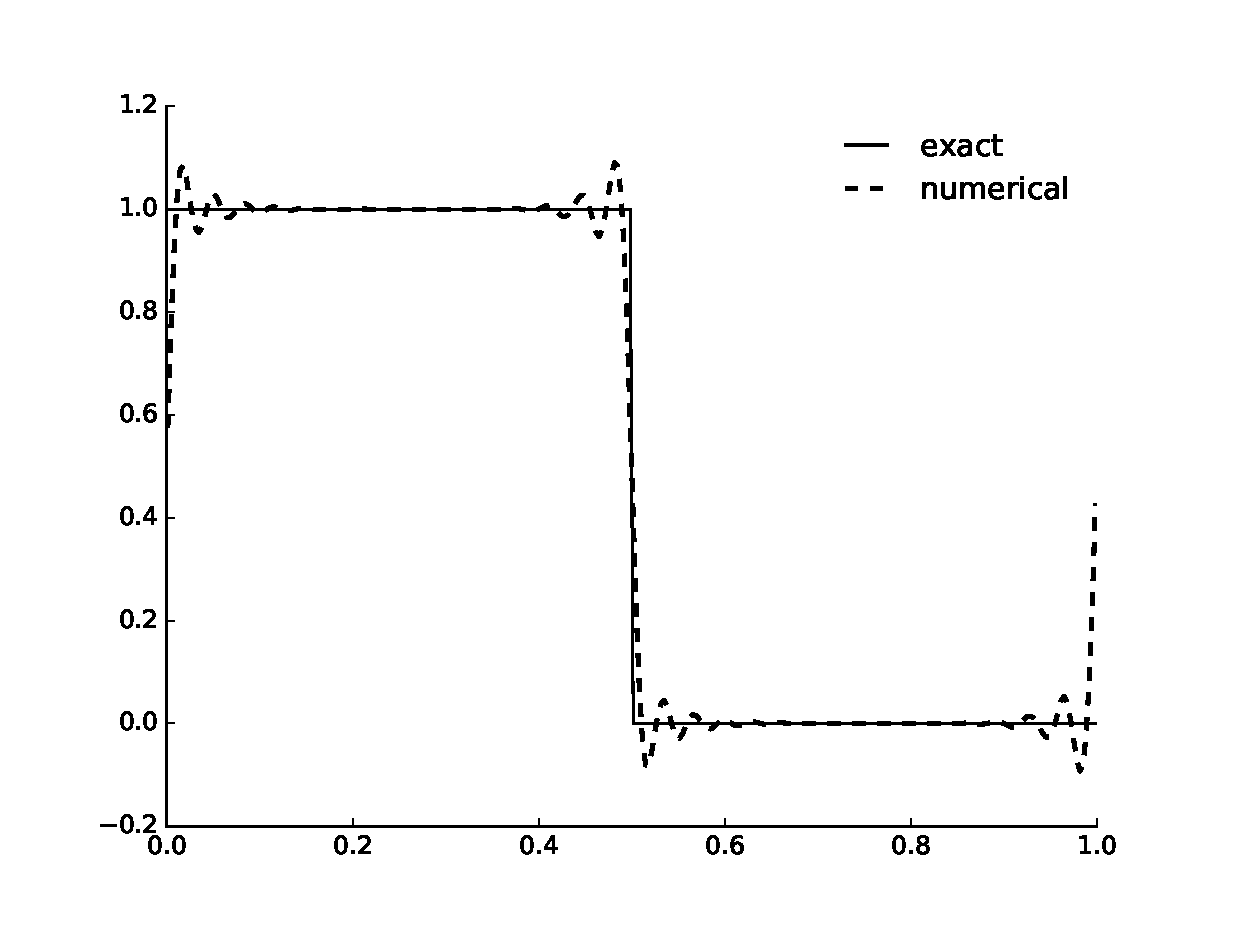
\includegraphics[width=0.8\columnwidth]{figures/oscillations}
  \caption{Linear advection of a shock solved with DG of order $p = 6$ on a grid of $20$ cells. The solution develops oscillations close to the discontinuities.}
  \label{fig:dg-oscillations}
\end{figure}

%%% -*- TeX-master: "case-study.tex" -*-
\section{The minmod limiter}
\label{sec:minmod}

Simulation of physical phenoma is an important use case for differential equation solvers, consequently ways to reduce or eliminate numerical errors have always been of interest.
One of the first ideas was researched by van Leer in 1979, when he proposed the $\minmod$ limiter\cite{VanLeer1979}.
A limiter in general restricts the steepness of the gradient of $U$ to sensible values where the bounds may be computed based on the current state or even set based on domain knowledge.
Of interest for us is in particular the former type because of its wide applicability.

The idea behind $\minmod$ specifically is to preserve the monotonicity of $U$.
% TODO: What is monotonicity? Does is provide TVD?
In the simplest case assume that the solution on cell $i$ is approximated by a first-order polynomial $c_{i}^{1}x + c_{i}^{0}$.
The limiter updates all the slopes $c_{i}^{1}$ to $\tilde{c}_{i}^{1}$ by
\begin{equation*}
  \tilde{c}_{i}^{1} = \minmod\left( c_{i}^{1}, \frac{c_{i + 1}^{0} - c_{i}^{0}}{\Delta x}, \frac{c_{i}^{0} - c_{i - 1}^{0}}{\Delta x} \right)
\end{equation*}
where the $\minmod$ operation is defined by
\begin{equation*}
  \minmod(a, b, c) = \begin{cases}
    \displaystyle\argmin_{x \in \{ a, b, c \}} |x| & \text{if} \sgn(a) = \sgn(b) = \sgn(c)\\
    0 & \text{otherwise}
  \end{cases}
\end{equation*}
So the slope on each cell is bounded by the forward and backward difference quotients of the cell and its neighbor's average values that approach the true first derivative as $\Delta x$ goes to $0$.
% TODO: How does this preserve monotonicity?

The effect of this limiter is demonstrated in figure \ref{fig:minmod}.
In figure \ref{fig:minmod-steep} the slope is limited so that the values do not exceed the average levels on neighboring cells.
Figure \ref{fig:minmod-extremum} shows how the approximation is reduced to first order in the case of an extremum as well as in the case that the slope does not agree with the trend set by the cell's neighbors (figure \ref{fig:minmod-trend}).
\begin{figure}[h]
  \centering
  \begin{subfigure}{0.5\columnwidth}
    \centering
    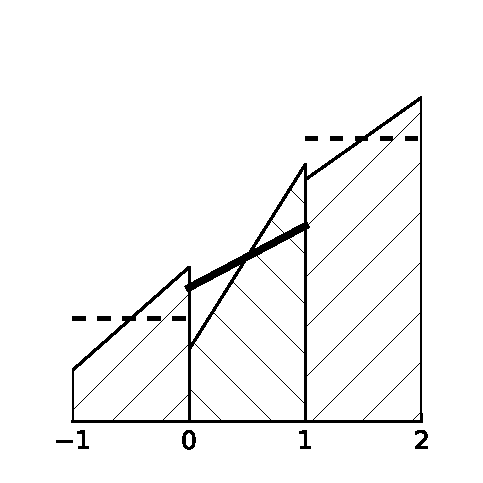
\includegraphics[width=\textwidth]{figures/minmod-a}
    \caption{Too steep}
    \label{fig:minmod-steep}
  \end{subfigure}
  \begin{subfigure}{0.5\columnwidth}
    \centering
    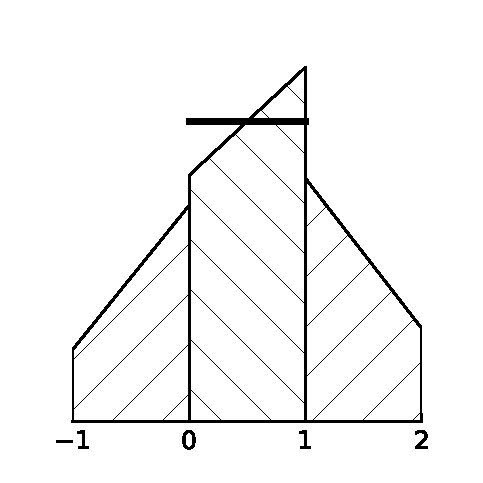
\includegraphics[width=\textwidth]{figures/minmod-b}
    \caption{Extremum in cell}
    \label{fig:minmod-extremum}
  \end{subfigure}
  \begin{subfigure}{0.5\columnwidth}
    \centering
    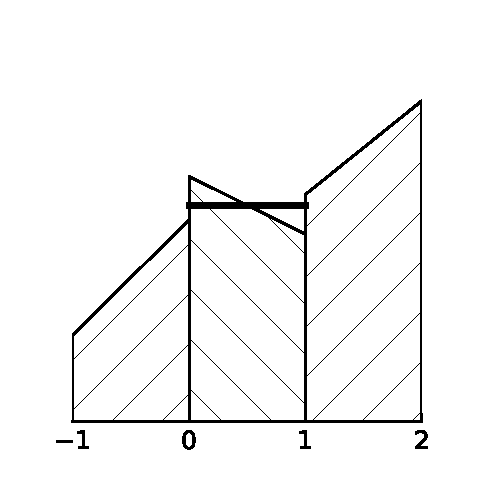
\includegraphics[width=\textwidth]{figures/minmod-c}
    \caption{Trend disagreement}
    \label{fig:minmod-trend}
  \end{subfigure}
  \caption{Three cell domain showcasing when the minmod limiter becomes active. Dashed line indicate average levels in a cell, bold lines designate limited slopes.}
  \label{fig:minmod}
\end{figure}

Prevent new extrema.
Generalization to higher orders.
reduces order to $1$.

%%% -*- TeX-master: "case-study.tex" -*-
\section{Total Variation}
\label{sec:total-variation}

In 1983 Harten published his theory on total variation diminishing methods \cite{Harten1983} that can be used to analyze a numerical method's ``oscillation-repressivity''.
A core concept of his work is the \emph{total variation} (TV) of a function, a way to measure the length of the graph of a function.
For an arbitrary function $f$ it is defined\cite[Sec. 6.7]{LeVequeFVMforHP} by
\begin{equation*}
  TV(f) = \sup_{\xi_{0}, \xi_{1}, \dots, \xi_{N}} \sum_{n = 1}^{N} |f(\xi_{n}) - f(\xi_{n - 1})|
\end{equation*}
where the $\xi_{n}$ form a partition of the domain of $f$, i.e. $\xi_{n - 1} < \xi_{n}$ and $\xi_{0}$ and $\xi_{N}$ are the left and right boundary of the domain of $f$.
Important properties are that the minimum is $0$ which is attained for constant $f$ and that the total variation grows as $f$ deviates more and more from a constant value, e.g. due to slopes and oscillations.
In particular the introduction of new extrema increases the total variation.

The connection to the weak solution of a differential equation is given by the property that the solution does not develop new extrema and the values of existing local minima are non-decreasing respectively the values of existing local maxima are non-increasing in time.
From this it follows that the solutions are \emph{total variation non-increasing} (TVNI) which is normally called \emph{total variation diminishing} (TVD) and means that the total variation of the solution is non-increasing in time.

There is actually a class of numerical schemes that will provably never produce unphysical extrema called \emph{monotone} schemes.
Unfortunately though, there is also a theorem by Godunov\cite{Godunov1959} that states that monotone schemes are at most first-order accurate.
So higher-order methods cannot be monotone but are nonetheless necessary for accurate results.

Harten showed that TVD is a relaxation of monotone in the sense that all monotone schemes are also TVD.
In addition he developed second-order methods that are TVD proving that the set of TVD schemes is a strict superset of monotone schemes and contains higher-order methods.
Consequently numerical methods should strive to produce TVD solutions to get as close to monotone as possible.

This brings us back to the $\minmod$ limiter.
Consider again Figures \ref{fig:minmod-extremum} and \ref{fig:minmod-trend}.
In the former the total variation is minimized by the $0$-slope because the increase in variation at the left boundary is counteracted by the decrease on the right side and on the interior the total variation is minimized by a constant function.
For the latter figure the same argument holds and it remains to argue why the slope in Figure \ref{fig:minmod-steep} is a fine choice.
Here the total variation is minimized by all slopes that agree with the trend set by the neighbors and are sufficiently flat that all values on the cell are bounded by the values on the neighboring cells.
So $\minmod$ is just one valid choice but nonetheless a minimizer.
Another valid choice would be to limit the slope to $0$ in all cases but that would reduce the accuracy to first order.

Although the $\minmod$ limiter is optimal in the sense that it makes schemes TVD, it is still lacking in various dimensions.
First, it is not directly extendable to higher-order solvers of order greater than $2$ which makes it incompatible with modern schemes.
Additionally it reduces the accuracy to first order in cells with extrema.
Both of these points are handled by the next limiter that we present in Section \ref{sec:moment}.
In contrast to $\minmod$ it is not TVD, yet numerical experiments suggest that it is at least total variation bounded, i.e. the solution's total variation does not grow without bounds.

%%% -*- TeX-master: "case-study.tex" -*-
\section{The generalized moment limiter}
\label{sec:moment}

The original moment limiter by Biswas et al. takes the idea from minmod to bound the gradient by the upwind and downwind difference quotient approximations to the first derivative and extends it to higher derivatives.
So the $k$-th derivative is bounded by the upwind and downwind difference quotients of the $k - 1$-th derivative in a manner that is to be further specified.
However, not all derivatives are limited in all cases.
Instead you start with the highest derivative and work your way down until a limiter is no longer \emph{active}, i.e. the limiter did not modify the value.
Krivodonova experimented with different variations but none of them worked as well as this top-down order.
For example limiting in the opposite order resulted in flattening of the extrema and limiting either all derivatives if at least one limiter was active or limiting none if not all limiters were active resulted in insufficient suppression of oscillations and reduced accuracy, respectively \cite[remark 1]{Krivodonova}.

The first important observation is that limiting the derivatives essentially amounts to limiting the coefficients of $U$.
We see this by taking the Taylor series expansion of the solution $u$ at $a$ on cell $i$
\begin{equation*}
  u(x, t') = \sum_{n = 0}^{\infty} \frac{(x - a)^{n}}{n!} \cdot \partial_{x}^{j} u(a, t')
\end{equation*}
and comparing it to $U_{i} = \sum_{j = 0}^{p} c_{i}^{j} P_{j}(x - a)$.
Equating the coefficients of the terms $(x - a)^{n}$ reveals
\begin{equation*}
  c_{i}^{j} \approx C \Delta x_{i} \partial_{x}^{j} u(x)
\end{equation*}
where $C$ is a constant scaling factor.

So limiting the derivatives and coefficients of $U$ amounts to the same thing.
Since we are extending the minmod limiter to higher derivatives, we are looking for an update formula for the coefficients of the form
\begin{equation*}
  \tilde{c}_{i}^{j} = \minmod(c_{i}^{j}, D_{i}^{+j}, D_{i}^{-j})
\end{equation*}
where $\tilde{c}_{i}^{j}$ is the limited $j$-th coefficient of $U_{i}$ and $D_{i}^{+k}$ and $D_{i}^{-k}$ are upwind respectively downwind first-order approximations to the $j$-th derivative.

We can work out feasible expressions for $D_{i}^{+k}$ and $D_{i}^{-k}$ by computing $U_{i}$s partial derivatives.
Note that the highest order coefficient of a Legendre polynomial $P_{j}$ written in the monomial basis is $\frac{(2j)!}{2^{j} j! j!}$.
Consequently its $j$-th derivative is given by
\begin{equation*}
  \partial_{x}^{j} P_{j}(x) = \frac{(2j)!}{2^{j} j! j!} \cdot j! = \frac{(2j)!}{2^{j} j!}
\end{equation*}
which we will use during the computation of the $k$-th derivative of $U_{i} \circ \xi_{i}$.
\begin{align}
  & \partial_{x}^{k} U_{i} \circ \xi_{i}(x) = \sum_{j = 0}^{p} c_{i}^{j} \partial_{x}^{k} P_{j}(\xi_{i}(x))\nonumber\\
  \intertext{The first $k - 1$ terms vanish since the $k + 1$-th derivative of a polynomial of degree $k$ is $0$.}
  =~& \sum_{j = k}^{p} c_{i}^{j} \partial_{x}^{k} P_{j}(\xi_{i}(x))\nonumber\\
  \intertext{Since the first derivative of $\xi_{i}$ is $\frac{2}{\Delta x_{i}}$, applying the chain rule $k$ times just pulls out this factor to the $k$-th power.}
  =~& \sum_{j = k}^{p} c_{i}^{j} \left( \frac{2}{\Delta x_{i}} \right)^{k} \partial_{\xi_{i}}^{k} P_{j}(\xi_{i}(x))\nonumber\\
  \intertext{Separating the first summand}
  =~& c_{i}^{k} \left( \frac{2}{\Delta x_{i}} \right)^{k} \partial_{\xi_{i}}^{k} P_{k}(\xi_{i}(x)) + \sum_{j = k + 1}^{p} c_{i}^{j} \left( \frac{2}{\Delta x_{i}} \right)^{k} \partial_{\xi_{i}}^{k} P_{j}(\xi_{i}(x))\nonumber\\
  \intertext{lets us plug in the $k$-th derivative of $P_{k}$}
  =~& c_{i}^{k} \left( \frac{2}{\Delta x_{i}} \right)^{k} \frac{(2k)!}{2^{k} k!} + \sum_{j = k + 1}^{p} c_{i}^{j} \left( \frac{2}{\Delta x_{i}} \right)^{k} \partial_{\xi_{i}}^{k} P_{j}(\xi_{i}(x))\nonumber\\
  \intertext{and simplify to}
  =~& c_{i}^{k} \left( \frac{2}{\Delta x_{i}} \right)^{k} \left( 2k - 1 \right)!! + \sum_{j = k + 1}^{p} c_{i}^{j} \left( \frac{2}{\Delta x_{i}} \right)^{k} \partial_{\xi_{i}}^{k} P_{j}(\xi_{i}(x)) \label{eq:kth-deriv}
\end{align}
where $!!$ is the double factorial, i.e. the factorial with all even factors cancelled out.

In the next step we approximate the $k$-th derivative with the forward and backward difference quotients.
Evaluating equation \eqref{eq:kth-deriv} for $k := k - 1$ yields the $k - 1$-th derivative of $U_{i} \circ \xi_{i}$
\begin{align*}
  \partial_{x}^{k - 1} U_{i} \circ \xi_{i}(x) & = c_{i}^{k - 1} \left( \frac{2}{\Delta x_{i}} \right)^{k - 1} \left( 2k - 3 \right)!!\\
  & \quad + \sum_{j = k}^{p} c_{i}^{j} \left( \frac{2}{\Delta x_{i}} \right)^{k - 1} \partial_{\xi_{i}}^{k - 1} P_{j}(\xi_{i}(x))
\end{align*}
By combining the values from neighboring cells we can compute the forward difference quotient
\begin{align}
  & \frac{\partial_{x}^{k - 1} U_{i + 1} \circ \xi_{i + 1} - \partial_{x}^{k - 1} U_{i} \circ \xi_{i}}{\Delta x}\nonumber\\
  =~& \left( \frac{2}{\Delta x} \right)^{k} \frac{(2k - 3)!!}{2} (c_{i + 1}^{k - 1} - c_{i}^{k - 1})\nonumber\\
  & + \frac{1}{2} \left( \frac{2}{\Delta x} \right)^{k} \sum_{j = k}^{p} (c_{i + 1}^{j} - c_{i}^{j}) \partial_{\xi_{i}}^{k - 1} P_{j}(\xi_{i}(x)) \label{eq:kth-deriv-forward}
\end{align}
and the backward difference quotient
\begin{align}
  & \frac{\partial_{x}^{k - 1} U_{i} \circ \xi_{i} - \partial_{x}^{k - 1} U_{i - 1} \circ \xi_{i - 1}}{\Delta x}\nonumber\\
  =~& \left( \frac{2}{\Delta x} \right)^{k} \frac{(2k - 3)!!}{2} (c_{i}^{k - 1} - c_{i - 1}^{k - 1})\nonumber\\
  & + \frac{1}{2} \left( \frac{2}{\Delta x} \right)^{k} \sum_{j = k}^{p} (c_{i}^{j} - c_{i - 1}^{j}) \partial_{\xi_{i}}^{k - 1} P_{j}(\xi_{i}(x)) \label{eq:kth-deriv-backward}
\end{align}
Note that this step only works on uniform meshes, i.e. $\Delta x_{i} = \Delta x_{j}~\forall i, j$, because otherwise you could not combine the $\frac{1}{\Delta x}$ factors.
Now we can get first order approximations to $c_{i}^{k}$ by equating the first summands of equations \eqref{eq:kth-deriv} and \eqref{eq:kth-deriv-forward} respectively \eqref{eq:kth-deriv} and \eqref{eq:kth-deriv-backward} and solving for $c_{i}^{k}$.
\begin{align*}
  c_{i}^{k} & \approx \frac{c_{i + 1}^{k - 1} - c_{i}^{k - 1}}{2(2k - 1)}\\
  c_{i}^{k} & \approx \frac{c_{i}^{k - 1} - c_{i - 1}^{k - 1}}{2(2k - 1)}
\end{align*}
By setting $D_{i}^{+k} = \frac{c_{i + 1}^{k - 1} - c_{i}^{k - 1}}{2(2k - 1)}$ and $D_{i}^{-k} = \frac{c_{i}^{k - 1} - c_{i - 1}^{k - 1}}{2(2k - 1)}$ we derive the moment limiter
\begin{equation*}
  \tilde{c}_{i}^{k} = \minmod\left( c_{i}^{k}, \frac{c_{i + 1}^{k - 1} - c_{i}^{k - 1}}{2(2k - 1)}, \frac{c_{i}^{k - 1} - c_{i - 1}^{k - 1}}{2(2k - 1)} \right)
\end{equation*}
However, numerical experiments by Krivodonova have shown that this is too diffusive.
% What does diffusive mean?
This is mitigated by equipping the differences with variable coefficients $\frac{1}{2(2k - 1)} \le \alpha_{i} \le 1$ and generalizing the limiter to
\begin{equation}
  \tilde{c}_{i}^{k} = \minmod\left( c_{i}^{k}, \alpha_{i} \left( c_{i + 1}^{k - 1} - c_{i}^{k - 1} \right), \alpha_{i} \left( c_{i}^{k - 1} - c_{i - 1}^{k - 1} \right) \right), \label{eq:moment-limiter}
\end{equation}
thus relaxing the limiter.
In further numerical tests by Krivodonova the best results where attained with the mildest limiter $\alpha_{i} = 1$.
This choice allows the coefficients to grow $2(2k - 1)$ times bigger than the first order approximations would suggest.
Yet the effectiveness of the limiter is not impaired since higher derivatives grow stronger near discontinuities while they have little weight in smooth portions.
Finally the choice $\alpha_{i} = 1$ makes it so that equation \eqref{eq:moment-limiter} reduces exactly to the original $\minmod$ definition for $p = 1$.

% Algorithmic summary (Maybe flowchart?)

%%% -*- TeX-master: "case-study.tex" -*-
\section{Numerical results}
\label{sec:results}

Krivodonova performed a series of tests to gather some insight into the limiter's behavior \cite[Section 4]{Krivodonova}.
Consider the linear advection problem
\begin{align*}
  & u_{t} + u_{x} = 0, \quad -1 \le x < 1, t > 0,\\
  & u(-1, t) = u(1, t), u(x, 0) = u_{0}(x)
\end{align*}
with symmetric boundary conditions where the initial value condition $u_{0}$ is given by a Gaussian bell curve, a square pulse, a sharp triangle and a half-ellipse distributed over the domain.
The exact solution would transport the initial condition across the domain while preserving the shape perfectly.
However, we would expect a numerical scheme with limiter to smear the discontinuities and reduce the height of sharp peaks over time.

\begin{figure}[h]
  \centering
  \begin{subfigure}[t]{0.48\columnwidth}
    \centering
    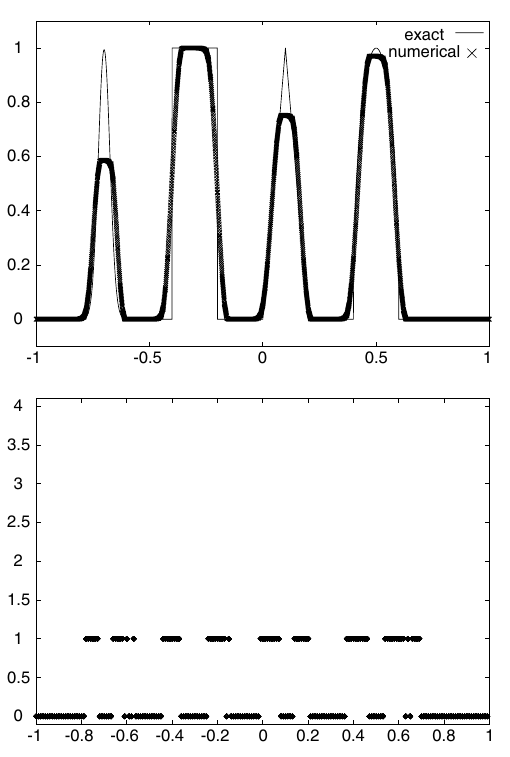
\includegraphics[width=\textwidth]{figures/moment-p-1}
    \caption{$p = 1$, moment limiter reduced to $\minmod$}
    \label{fig:results-advection-p1}
  \end{subfigure}
  \hfill
  \begin{subfigure}[t]{0.48\columnwidth}
    \centering
    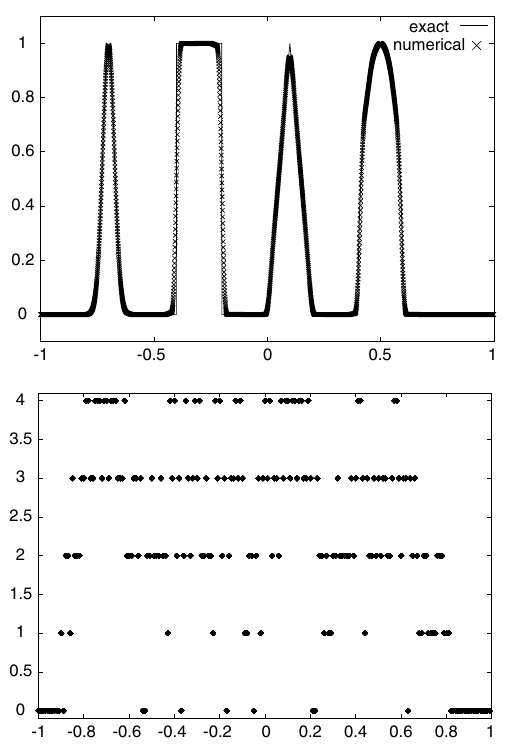
\includegraphics[width=\textwidth]{figures/moment-p-4}
    \caption{$p = 4$, with full moment limiter}
    \label{fig:results-advection-p4}
  \end{subfigure}
  \caption{Linear advection of various shapes on $200$ cells. Top part shows exact and numerical solutions while bottom part shows limiter activity. \cite[Figure 2]{Krivodonova}}
  \label{fig:results-advection}
\end{figure}

The results are displayed in Figure \ref{fig:results-advection}.
Figure \ref{fig:results-advection-p1} shows the results for $p = 1$ and Figure \ref{fig:results-advection-p4} shows the results for $p = 4$, whereas in both figures the top part is a plot of the current state and the bottom part indicates limiter activity.
A dot in the activity plot marks the highest coefficient that was not limited, e.g. a point at 2 means that coefficients $3$ and $4$ were limited.

In the case of $p = 1$ the moment limiter which is identical to $\minmod$ here, behaves as expected.
The discontinuities have been noticeably smeared and a good portion of the height of the sharp peaks has been limited away.
At the same time though any oscillations were successively prevented.
The results for the fourth-order polynomials -- and thus fourth-order moment limiter -- came out better by all accounts.
There is no loss of height visible for the Gaussian bell shape as well as the half-ellipse and it has been reduced for the triangle.
Furthermore the approximations to the discontinuities have remained steeper and the corners on the square pulse are less rounded.
It is important to see that these improvements did not arise from the increase in polynomial degree but from the fact that the moment limiter discards less information.
$\minmod$ applied to fourth degree polynomials would limit the result to a similar degree as shown in Figure \ref{fig:results-advection-p1}.

The activity plots are not as easily digestible.
In the first-order case we see that the limiter is not active in areas where the exact solution has steep gradients.
So there the coefficients are naturally bounded by the first-order approximations.
Curiously, the limiter is active in the flat regions.
A possible explanation is that the DG solver erroneously produces polynomial coefficients for higher degrees on the order of machine precision which are then bounded by difference quotients that are truly equal to $0$.
For $p = 4$ the activity plot shows that all four levels of limiting are used across the domain.
Additionally it extends the phenomenon from the first case to higher-order case that the limiter is most aggressive in flat regions and most permissive in the vicinity of steep gradients.

%%% -*- TeX-master: "case-study.tex" -*-
\section{Conclusion and Outlook}
\label{sec:conclusion}

We have presented the generalized moment limiter for discontinuous Galerkin methods together with its foundation, the minmod limiter, and looked into numerical results, that showcase the limiters utility and effectiveness.

The limiter has further potential for theoretical analysis as well as transfer to related methods.
One should work out the details of the connection between the coefficients and the derivatives of the Legendre polynomials, since such an analysis could yield more insight into the choice of limiter parameters.
Alternatively one could try to use a different set of basis functions.
There could be a candidate for which the aforementioned connection can be more easily determined.
Related to the search for promising basis functions is the idea of building a high-order limiter for nodal DG methods.


%%%%%%%%%%%%%%%%%%%%%%%%%%%%%%%%%%%%%%%%%%%%%%%%%%%%%%%%%%%%%%%%%%%%%%%%%%
% 	Acknowledgements
%%%%%%%%%%%%%%%%%%%%%%%%%%%%%%%%%%%%%%%%%%%%%%%%%%%%%%%%%%%%%%%%%%%%%%%%%%

%\section*{Acknowledgment}
%\addcontentsline{toc}{section}{Acknowledgment}

%%%%%%%%%%%%%%%%%%%%%%%%%%%%%%%%%%%%%%%%%%%%%%%%%%%%%%%%%%%%%%%%%%%%%%%%%%
% 	References
%%%%%%%%%%%%%%%%%%%%%%%%%%%%%%%%%%%%%%%%%%%%%%%%%%%%%%%%%%%%%%%%%%%%%%%%%%

% trigger a \newpage just before the given reference
% number - used to balance the columns on the last page
% adjust value as needed - may need to be readjusted if
% the document is modified later
%\IEEEtriggeratref{8}
% The "triggered" command can be changed if desired:
%\IEEEtriggercmd{\enlargethispage{-5in}}

% references section
% NOTE: BibTeX documentation can be easily obtained at:
% http://www.ctan.org/tex-archive/biblio/bibtex/contrib/doc/

% can use a bibliography generated by BibTeX as a .bbl file
% standard IEEE bibliography style from:
% http://www.ctan.org/tex-archive/macros/latex/contrib/supported/IEEEtran/bibtex
\bibliographystyle{IEEEtran}
% argument is your BibTeX string definitions and bibliography database(s)
\bibliography{IEEEabrv,references}
%
% <OR> manually copy in the resultant .bbl file
% set second argument of \begin to the number of references
% (used to reserve space for the reference number labels box)
%\begin{thebibliography}{1}
%
%\bibitem{ref:kopka}
%H.~Kopka and P.~W. Daly, \emph{A Guide to {\LaTeX}}, 3rd~ed.\hskip 1em plus
%  0.5em minus 0.4em\relax Harlow, England: Addison-Wesley, 1999.
%
%\end{thebibliography}

%%%%%%%%%%%%%%%%%%%%%%%%%%%%%%%%%%%%%%%%%%%%%%%%%%%%%%%%%%%%%%%%%%%%%%%%%%
% 	End of the document
%%%%%%%%%%%%%%%%%%%%%%%%%%%%%%%%%%%%%%%%%%%%%%%%%%%%%%%%%%%%%%%%%%%%%%%%%%

\end{document}
